
% Festlegung des Allgemeinen Dokumentenformats
\documentclass[a4paper,12pt,headsepline]{scrartcl}
% Umlaute unter UTF8 nutzen
\usepackage[utf8]{inputenc}
% Variablen
%Variablen welche innerhalb der gesamten Arbeit zur Verfügung stehen sollen
\newcommand{\titleDocument}{Seminararbeit}
\newcommand{\subjectDocument}{Generative Modelle im maschinellen Lernen}

% weitere Pakete
% Grafiken aus PNG Dateien einbinden
\usepackage{graphicx}
% Deutsche Sonderzeichen und Silbentrennung nutzen
\usepackage[ngerman]{babel}
% Eurozeichen einbinden
\usepackage[right]{eurosym}
% Zeichenencoding
\usepackage[T1]{fontenc}
\usepackage{lmodern}
% floatende Bilder ermöglichen
%\usepackage{floatflt}
% mehrseitige Tabellen ermöglichen
\usepackage{longtable}
% Unterstützung für Schriftarten
%\newcommand{\changefont}[3]{ 
%\fontfamily{#1} \fontseries{#2} \fontshape{#3} \selectfont}
% Packet für Seitenrandabständex und Einstellung für Seitenränder
\usepackage{geometry}
\geometry{left=3.5cm, right=2cm, top=2.5cm, bottom=2cm}

% Paket für Boxen im Text
\usepackage{fancybox}

% bricht lange URLs "schön" um
\usepackage[hyphens,obeyspaces,spaces]{url}

% Paket für Textfarben
\usepackage{color}

% Mathematische Symbole importieren
\usepackage{amssymb, amsmath}

% auf jeder Seite eine Überschrift (alt, zentriert)
%\pagestyle{headings}

% erzeugt Inhaltsverzeichnis mit Querverweisen zu den Abschnitten (PDF Version)
\usepackage[bookmarksnumbered,pdftitle={\titleDocument},hyperfootnotes=false, hidelinks]{hyperref}
%\hypersetup{colorlinks, citecolor=red, linkcolor=blue, urlcolor=black}
%\hypersetup{colorlinks, citecolor=black, linkcolor= black, urlcolor=black}

% neue Kopfzeilen mit fancypaket
\usepackage{fancyhdr} %Paket laden
\pagestyle{fancy} %eigener Seitenstil
\fancyhf{} %alle Kopf- und Fußzeilenfelder bereinigen
\fancyhead[L]{\nouppercase{\leftmark}} %Kopfzeile links
\fancyhead[C]{} %zentrierte Kopfzeile
\fancyhead[R]{\thepage} %Kopfzeile rechts
\renewcommand{\headrulewidth}{0.4pt} %obere Trennlinie
%\fancyfoot[C]{\thepage} %Seitennummer
%\renewcommand{\footrulewidth}{0.4pt} %untere Trennlinie

% für Tabellen
\usepackage{array}

% Runde Klammern für Zitate
%\usepackage[numbers,round]{natbib}

% Festlegung Art der Zitierung - Havardmethode: Abkuerzung Autor + Jahr
\bibliographystyle{alphadin}

% Schaltet den zusätzlichen Zwischenraum ab, den LaTeX normalerweise nach einem Satzzeichen einfügt.
%\frenchspacing

% Paket für Zeilenabstand
\usepackage{setspace}

% für Bildbezeichner
\usepackage{capt-of}

% für Stichwortverzeichnis
\usepackage{makeidx}

% für Listings
%\usepackage{listings}
%\lstset{numbers=left, numberstyle=\tiny, numbersep=5pt, keywordstyle=\color{black}\bfseries, stringstyle=\ttfamily,showstringspaces=false,basicstyle=\footnotesize,captionpos=b}
%\lstset{language=java}

% Indexerstellung
\makeindex

% Abkürzungsverzeichnis
\usepackage[german]{nomencl}
\let\abbrev\nomenclature

% Abkürzungsverzeichnis LiveTex Version
% Titel des Abkürzungsverzeichnisses
\renewcommand{\nomname}{Abkürzungsverzeichnis}
% Abstand zwischen Abkürzung und Erläuterung
\setlength{\nomlabelwidth}{.25\textwidth}
% Zwischenraum zwischen Abkürzung und Erläuterung mit Punkten
\renewcommand{\nomlabel}[1]{#1 \dotfill}
% Variation des Abstandes der einzelnen Abkürzungen zu einander
\setlength{\nomitemsep}{-\parsep}
% Index mit Abkürzungen erzeugen
\makenomenclature
%\makeglossary

% Abkürzungsverzeichnis TeTEX Version
% \usepackage[german]{nomencl}
% \makenomenclature
% %\makeglossary
% \renewcommand{\nomname}{Abkürzungsverzeichnis}
% \AtBeginDocument{\setlength{\nomlabelwidth}{.25\columnwidth}}
% \renewcommand{\nomlabel}[1]{#1 \dotfill}
% \setlength{\nomitemsep}{-\parsep}

% Optional: Einzelne Zeilen am Anfang einer Seite unterdrücken (Schusterjungen)
% \clubpenalty = 10000
% Optional: Einzelne Zeilen am Ende einer Seite unterdrücken (Hurenkinder)
% \widowpenalty = 10000
% \displaywidowpenalty = 10000

\begin{document}
% hier werden die Trennvorschläge inkludiert
%hier müssen alle Wörter rein, welche Latex von sich auch nicht korrekt trennt bzw. bei denen man die genaue Trennung vorgeben möchte
\hyphenation{
Film-pro-du-zen-ten
Lux-em-burg
Soft-ware-bau-steins
zeit-in-ten-siv
}


% Schriftart Helvetica verwenden
%\usepackage{helvet}
%\renewcommand\familydefault{\sfdefault}

% Leere Seite am Anfang
%\thispagestyle{empty} % erzeugt Seite ohne Kopf- / Fusszeile
%\mbox{}
%\newpage

% Titelseite %
\thispagestyle{empty}


%\SetWatermarkText{Vorabversion}
%\SetWatermarkScale{3}
%\SetWatermarkColor[gray]{0.9}
%\SetWatermarkFontSize{1cm}

\begin{figure}[t]
 \raggedleft
 
\includegraphics[width=0.4\textwidth]{abb/BHT_Logo}
 %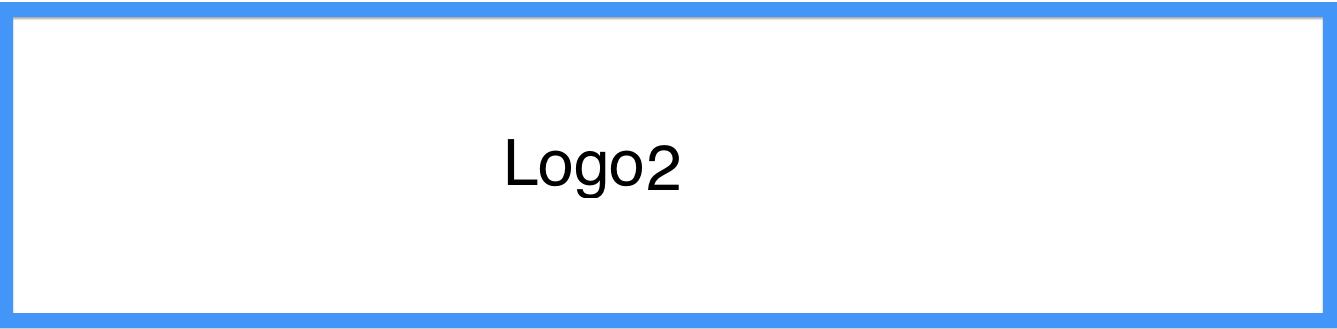
\includegraphics[width=0.3\textwidth]{abb/logo2}
\end{figure}
\begin{center}
\end{center}
\vspace{2cm}
\begin{center}
\Large{Beuth Hochschule für Technik}\\
\end{center}
\begin{center}
\vspace{3cm}
\end{center}
\begin{center}
\doublespacing
\textbf{\LARGE{\titleDocument}}
\singlespacing

\textbf{Einführung in die wissenschaftliche Projektarbeit}
\end{center}
%\vspace{8cm}
\vfill
\begin{flushleft}
\begin{tabular}{llll}
\textbf{Thema:} & & {\subjectDocument} & \\
& & \\
\textbf{Autor:} & & Frank Trojanowski <info@franktrojanowski.com>& \\
& & Matrikelnummer: 881001 & \\
& & \\
\textbf{Version vom:} & & \today &\\
& & \\
\textbf{Betreuer:} & & Dr. Hussein Hussein &\\
\end{tabular}
\end{flushleft}

% römische Numerierung
\pagenumbering{roman}

% 1.5 facher Zeilenabstand
\onehalfspacing

\newpage
% Einleitung / Abstract
\thispagestyle{empty}
\section*{Kurzfassung}

Hier steht der Text, welcher den Inhalte der Seminararbeit zusammenfasst...

Lorem ipsum dolor sit amet, consetetur sadipscing elitr, sed diam nonumy eirmod tempor invidunt ut labore et dolore magna aliquyam erat, sed diam voluptua. At vero eos et accusam et justo duo dolores et ea rebum. Stet clita kasd gubergren, no sea takimata sanctus est Lorem ipsum dolor sit amet. Lorem ipsum dolor sit amet, consetetur sadipscing elitr, sed diam nonumy eirmod tempor invidunt ut labore et dolore magna aliquyam erat, sed diam voluptua. At vero eos et accusam et justo duo dolores et ea rebum. Stet clita kasd gubergren, no sea takimata sanctus est Lorem ipsum dolor sit amet.

\section*{Abstract}

Lorem ipsum dolor sit amet, consetetur sadipscing elitr, sed diam nonumy eirmod tempor invidunt ut labore et dolore magna aliquyam erat, sed diam voluptua. At vero eos et accusam et justo duo dolores et ea rebum. Stet clita kasd gubergren, no sea takimata sanctus est Lorem ipsum dolor sit amet. Lorem ipsum dolor sit amet, consetetur sadipscing elitr, sed diam nonumy eirmod tempor invidunt ut labore et dolore magna aliquyam erat, sed diam voluptua. At vero eos et accusam et justo duo dolores et ea rebum. Stet clita kasd gubergren, no sea takimata sanctus est Lorem ipsum dolor sit amet.


% einfacher Zeilenabstand
\singlespacing

\newpage
% Seitenzählung bei Inhaltsverzeichnis beginnen
\setcounter{page}{1}

% Inhaltsverzeichnis anzeigen
\thispagestyle{empty}
\tableofcontents

\newpage
% das Abbildungsverzeichnis
% Abbildungsverzeichnis soll im Inhaltsverzeichnis auftauchen
\addcontentsline{toc}{section}{Abbildungsverzeichnis}
% Verion 1: Abbildungsverzeichnis MIT führender Nummberierung endgueltig anzeigen
\listoffigures

% Verion 2: Abbildungsverzeichnis OHNE führende Nummberierung endgueltig anzeigen
%\begingroup
%\renewcommand\numberline[1]{}
%\listoffigures
%\endgroup

% das Tabellenverzeichnis
%\newpage
% Tabellenverzeichnis soll im Inhaltsverzeichnis auftauchen
%\addcontentsline{toc}{section}{Tabellenverzeichnis}
% \fancyhead[L]{Abbildungsverzeichnis / Abkürzungsverzeichnis} %Kopfzeile links
% Tabellenverzeichnis endgültig anzeigen
%\listoftables

%% WORKAROUND für Listings
%\makeatletter% --> De-TeX-FAQ
%\renewcommand*{\lstlistoflistings}{%
%  \begingroup
%    \if@twocolumn
%      \@restonecoltrue\onecolumn
%    \else
%      \@restonecolfalse
%    \fi
%    \lol@heading
%    \setlength{\parskip}{\z@}%
%    \setlength{\parindent}{\z@}%
%    \setlength{\parfillskip}{\z@ \@plus 1fil}%
%    \@starttoc{lol}%
%    \if@restonecol\twocolumn\fi
%  \endgroup
%}
%\makeatother% --> \makeatletter
% das Listingverzeichnis
\newpage
% Listingverzeichnis soll im Inhaltsverzeichnis auftauchen
%\addcontentsline{toc}{section}{Listingverzeichnis}
%\fancyhead[L]{Listingverzeichnis} %Kopfzeile links
%\renewcommand{\lstlistlistingname}{Listingverzeichnis}
%\lstlistoflistings


% das Abkürzungsverzeichnis
\newpage
% Abkürzungsverzeichnis soll im Inhaltsverzeichnis auftauchen
\addcontentsline{toc}{section}{Abkürzungsverzeichnis}
% das Abkürzungsverzeichnis ausgeben
\fancyhead[L]{Abkürzungsverzeichnis} %Kopfzeile links
\nomenclature{GAN}{Generative Adversarial Network}
\nomenclature{NN}{Neural Network}
\nomenclature{CNN}{Convolutional Neural Network}
\nomenclature{RNN}{Recurrent Neural Network}
\nomenclature{VAE}{Variational Autoencoder}
\nomenclature{KI}{Künstliche Intelligenz}
\nomenclature{AI}{Artificial Intelligence}
\nomenclature{ML}{Machine Learning}
\nomenclature{KNN}{Künstliches Neurales Netz}
\nomenclature{LSTM}{Long Short-Term Memory}
\nomenclature{NIPS}{Neural Information Processing Systems (Konferenz)}
\nomenclature{DCGAN}{Deep Convolutional Generative Adversarial Networks}
\nomenclature{KL-Divergenz}{Kullback-Leibler-Divergenz}
\nomenclature{SRGAN}{Super Resolution Generative Adversarial Network}
\nomenclature{DCGAN}{Deep Convolutional Generative Adversarial Network}


\printnomenclature[3cm]


%%%%%%% EINLEITUNG %%%%%%%%%%%%
\newpage
\fancyhead[L]{\nouppercase{\leftmark}} %Kopfzeile links

% 1,5 facher Zeilenabstand
\onehalfspacing

% arabische Seitennummerierung ab hier
\pagenumbering{arabic}

% einzelne Kapitel werden hier eingebunden
\section{Einführung in Machine Learning}\label{Machine Learning}
Machine Learning (ML) ist ein interdisziplinäres Teilgebiet der künstlichen Intelligenz, welches die Generierung von »Wissen« aus »Erfahrung« bezweckt. Mithilfe von ML werden IT-Systeme in die Lage versetzt, auf Basis vorhandener Datenbestände und Algorithmen Muster und Gesetzmäßigkeiten zu erkennen und ein komplexes Modell der Daten zu entwickeln. Das Modell, und damit die automatisch erworbene Wissensrepräsentation, kann dann verallgemeinert für neue Problemlösungen oder für die Analyse von bisher unbekannten Daten verwendet werden. Dazu verwendet ML zahlreiche Methoden, wobei in vorliegender Seminararbeit nur jene erläutert werden, welche für das allgemeine Verständnis generativer Modelle nötig sind.
%\cite{mm2009}

\subsection{Deep Learning}\label{Deep Learning}
%$p_{model}$, $p_{model}$ $\boldsymbol{\hat{\theta}}$
%\textsl{Lorem} 
Deep Learning umfasst eine Reihe von Algorithmen, deren Architektur auf mehreren nacheinander angeordneten Verarbeitungsschichten basiert und deren Aufgabe es ist, aus unstrukturierten Daten übergeordnete Repräsentationen zu lernen.
Deep-Learning-Modelle können auf strukturierte Daten angewendet werden, aber ihre eigentliche Stärke, insbesondere im Hinblick auf die generative Modellierung, ergibt sich aus ihrer Fähigkeit, unstrukturierte Daten verarbeiten zu können. In den meisten Fällen liegt es in der Natur der Aufgabe, unstrukturierte Daten wie neue Bilder oder echte Textzeilen zu erzeugen. Daher verwundert es wenig, dass vor allem die Entwicklungen im Deep Learning einen bedeutenden Einfluss auf die generative Modellierung hatten\cite{fos19}.
Bei der Mehrheit aller Deep-Learning-Modelle handelt es sich um künstliche neuronale Netze (KNNs, kurz »neuronale Netze«) mit mehreren hintereinanderliegenden verborgenen Schichten. Aus diesem Grund ist Deep Learning inzwischen fast zum Synonym für tiefe neuronale Netzwerke geworden. Es ist jedoch wichtig darauf hinzuweisen, dass jedes System, das mehrere Schichten verwendet, um übergeordnete Darstellungen der Eingangsdaten zu lernen, auch eine Form des Deep Learning ist (z. B. Deep-Believe-Netzwerke und Deep-Boltzmann-Maschinen).
Um Annahmen nicht bereits im Voraus treffen zu müssen, wird ein Modell benötigt, das die relevanten Strukturen aus den Daten selbst ableiten kann. Hierbei zeichnet sich Deep Learning aus. Die Tatsache, dass Deep Learning seine eigenen Merkmale in einem niederdimensionalen Raum finden kann, bedeutet eine Form des \hyperref[Representation Learning]{Representation Learnings}\cite{goodl16}.

\subsection{überwachtes und unüberwachtes Lernen}\label{überwachtes / unüberwachtes Lernen}
Wenn ein Modell anhand gekennzeichneter Trainingsdaten (\emph{labeled data}) lernen soll, handelt es sich um überwachtes Lernen. Die Methode richtet sich also nach einer im Vorhinein festgelegten Ausgabe, deren Ergebnisse bekannt sind. Die Ergebnisse des Lernprozesses können mit den bekannten, richtigen Ergebnissen verglichen, also überwacht, werden. Die Überwachung bezieht sich dabei nur auf die sogenannten Trainingsdaten, mit denen ein KNN für die Lösung einer Aufgabe trainiert wird. Im produktiven Einsatz des Modells wird grundsätzlich nicht überwacht.
Zu den überwachten Lernverfahren zählen alle Verfahren zur Klassifikation oder Regression, beispielsweise mit Algorithmen wie k-nearest-Neighbour, Random Forest, Support Vector Machines oder auch Verfahren der Dimensionsreduktion wie die lineare Diskriminanzanalyse. Der Nachteil von überwachtem Lernen besteht jedoch in einem oft sehr hohen manuellen Aufwand bei der Aufbereitung der Trainingsdaten.
Eine besondere Form des überwachten Lernens ist die des bestärkenden Lernens. Bestärkendes Lernen kommt dann zum Einsatz, wenn ein Endergebnis noch nicht bestimmbar ist, jedoch der Trend hin zum Erfolg oder Misserfolg erkennbar wird. In der Trainingsphase werden beim bestärkenden Lernen die korrekten Ergebnisse also nicht zur Verfügung gestellt, jedoch wird jedes Ergebnis bewertet, ob dieses (wahrscheinlich) in die richtige oder falsche Richtung geht.\cite{ras18}

Im Gegensatz zum überwachten Lernen werden beim unüberwachten Lernen weder gekennzeichnete, noch klassifizierte Trainingsdaten verwendet. Ziel dieses Ansatzes ist es, aus den Daten unbekannte Muster zu erkennen und Regeln aus diesen abzuleiten. Das ML-System nutzt Algorithmen, die die Struktur der Eingabedaten erkunden und daraus sinnvolle Informationen in den Ausgabedaten abbilden. Die Vorteile des unüberwachten Lernens bestehen in der teilweise vollautomatisierten Erstellung von Modellen. Dabei können diese eine sehr gute Prognose über neue Daten hervorbringen oder gar neue Inhalte erstellen (generative Modelle). Das Modell lernt mit jedem neuen Datensatz dazu und verfeinert gleichzeitig seine Berechnungen und Klassifizierungen. Ein manueller Eingriff ist dadurch nicht mehr notwendig. KNNs basieren auf diesem selbstlernenden Verfahren.

\subsection{Representation Learning}\label{Representation Learning}
Die Grundidee beim Lernen von Repräsentationen besteht darin, nicht den hochdimensionalen Stichprobenraum direkt zu modellieren, sondern jede Beobachtung im Trainingsdatensatz mittels eines niederdimensionalen latenten Raums zu erfassen. Das Modell muss dann eine Mapping-Funktion lernen, die einen Punkt im latenten Raum nehmen und ihn auf einen Punkt in dem ursprünglichen Raum abbilden kann. Mit anderen Worten: Jeder Punkt im latenten Raum ist die Darstellung einer hochdimensionalen Repräsentation der Eingabedaten, beispielsweise eines Bilds.



%\subsection{überwachtes und unüberwachtes Lernen}\label{überwachtes und unüberwachtes Lernen}
%Hier steht die Einleitung der Arbeit... Lorem ipsum dolor sit amet, consetetur sadipscing elitr, sed diam nonumy eirmod tempor invidunt ut labore et dolore magna aliquyam erat, sed diam voluptua. At vero eos et accusam et justo duo dolores et ea rebum. Stet clita kasd gubergren, no sea takimata sanctus est Lorem ipsum dolor sit amet. Lorem ipsum dolor sit amet, consetetur sadipscing elitr, sed diam nonumy eirmod tempor invidunt ut labore et dolore magna aliquyam erat, sed diam voluptua. At vero eos et accusam et justo duo dolores et ea rebum. Stet clita kasd gubergren, no sea takimata sanctus est Lorem ipsum dolor sit amet.
\newpage

\section{Generative Modelle}\label{Generative Modelle}
%ein generatives Modell $p_{model}$, $p_{data}$
Ein generatives Modell beschreibt, wie ein Datensatz im Rahmen eines Wahrscheinlichkeitsmodells erzeugt wird. Die aus diesem Modell gewonnenen Stichproben ermöglichen es, neue Daten zu generieren.

Gegeben sei ein Datensatz mit Bildern von bestimmten Objekten. Es soll ein Modell entwickelt werden, das ein neues Bild von einem dieser Objekte erzeugen kann, das nie existiert hat, aber trotzdem realistisch aussieht. Dies ist möglich, weil das Modell die allgemeinen Prinzipien gelernt hat, die das Aussehen dieses Objektes bestimmen. Genau dies ist die Form von Aufgabenstellung, die sich mithilfe eines generativen Modells im Machine Learning lösen lässt \cite[vgl. S. 54]{fos19}.
Zuerst benötigt man einen Datensatz, der aus zahlreichen Beispielen der zu erzeugenden Entität besteht. Man spricht in diesem Zusammenhang vom Trainingsdatensatz, bei dem jeder der Eingabedatenpunkte als Beobachtung bezeichnet wird.
Jede Beobachtung besteht aus vielen Merkmalen – bei einer Bilderzeugungsaufgabe sind die Merkmale üblicherweise die jeweiligen Werte der einzelnen Pixel. Das Ziel ist es, ein Modell zu erstellen, das neue Merkmale erzeugen kann, die so aussehen, als wären sie nach den gleichen Regeln wie die Originaldaten erstellt worden. Rein konzeptionell ist dies für die Bilderzeugung eine unglaublich schwierige Aufgabe – bedenkt man, wie vielfältig die einzelnen Pixelwerte zugeordnet werden können und wie vergleichsweise gering dagegen die Anzahl der Anordnungen ist, die ein Bild der Entität erzeugen, die reproduziert werden soll.

Ein generatives Modell sollte zudem probabilistisch und nicht deterministisch sein. Wenn das Modell nur eine fest vorgegebene Berechnung umfasst, wie z. B. die Berechnung des Durchschnittswerts jedes Pixels im Datensatz, ist es nicht generativ, da das Modell jedes Mal die gleiche Ausgabe erzeugt. Folglich muss das Modell ein stochastisches (zufälliges) Element beinhalten, das die von ihm erzeugten Ausgaben beeinflusst.
Es gibt also eine unbekannte Wahrscheinlichkeitsverteilung, die erklärt, warum einige Bilder wahrscheinlich im Trainingsdatensatz zu finden sind und andere Bilder hingegen nicht. Es muss ein Modell entwickelt werden, das diese Verteilung so genau wie möglich nachahmt, um daraus neue, einzigartige Beobachtungen zu generieren, die so aussehen, als würden sie dem ursprünglichen Trainingsdatensatz entstammen. In diesem Kapitel sollen zwei Beispiele der meistgenutzten generativen Modelle erläutert werden.

\subsection{Vergleich diskriminativer und generativer Modelle}\label{Vergleich diskriminativer und generativer Modelle}
Um zu verstehen, was generative Modelle leisten sollen und warum sie wichtig sind, ist es sinnvoll, sie mit ihrem Gegenstück, den diskriminativen Modellen, zu vergleichen. Die meisten Fragestellungen im ML sind diskriminativer Natur.

Ein wesentlicher Unterschied besteht darin, dass bei diskriminativen Modellen jede Beobachtung in den Trainingsdaten mit einem Label versehen ist. Im Fall einer binären Klassifikationsaufgabe wären beispielsweise Gemälde von Picasso mit einer 1 und alle anderen mit einer 0 gekennzeichnet. Das Modell lernt dann, beide Gruppen zu unterscheiden, und gibt die Wahrscheinlichkeit aus, dass eine neue Beobachtung das Label 1 trägt – gleichbedeutend damit, dass sie von Picasso gemalt wurde.\cite{fos19}
Deshalb ist diskriminative Modellierung synonym mit überwachtem Lernen beziehungsweise dem Erlernen einer Funktion, die eine Eingabe mithilfe eines mit Labeln versehenen Datensatzes auf eine Ausgabe abbildet.
Für generative Modelle bedarf es für gewöhnlich nur ungelabelter Datensätze (als Form des unüberwachten Lernens). Sie kann jedoch auch auf einen mit Labeln versehenen Datensatz angewendet werden, um zu lernen, wie man Beobachtungen und Merkmale aus den einzelnen Kategorien erzeugt.

\subsection{Variational Autoencoders (VAE)}\label{Variational Autoencoders (VAE)}
Im Vergleich zu den diskriminativen Aufgaben von KNN als Regressoren und Klassifikatoren haben VAEs starke generative Modelle, die mittlerweile diverse Anwendungsmöglichkeiten haben, von der Erzeugung menschlicher Gesichter bis zur Produktion reinsynthetischer Musik. Dabei möchte man aber meist bereits vorhandene Daten nicht auf zufällige Weise verändern, sondern die erzeugten Ausgaben in eine spezifische Richtung steuern. VAEs sind in dieser Hinsicht allen anderen momentan bekannten Methoden überlegen. Um die Funktionsweise von VAEs zu verstehen, ist es hilfreich, sich erst einmal einen Standard-Autoencoder anzuschauen:

\subsubsection{Autoencoder}~\\
Ein Autoencoder-Netzwerk ist eigentlich ein in Encoder und Decoder geteiltes KNN. Der Encoder nimmt Eingabedaten und konvertiert diese in eine kleinere, dichtere Repräsentation. Das Encoding beschreibt die komprimierten Daten im latenten Raum. Der Decoder kann die ursprünglichen Daten fast originalgetreu aus dieser Repräsentation wiederherstellen \cite[S.499ff]{goodl16}.
\begin{figure}[H]
    \centering
    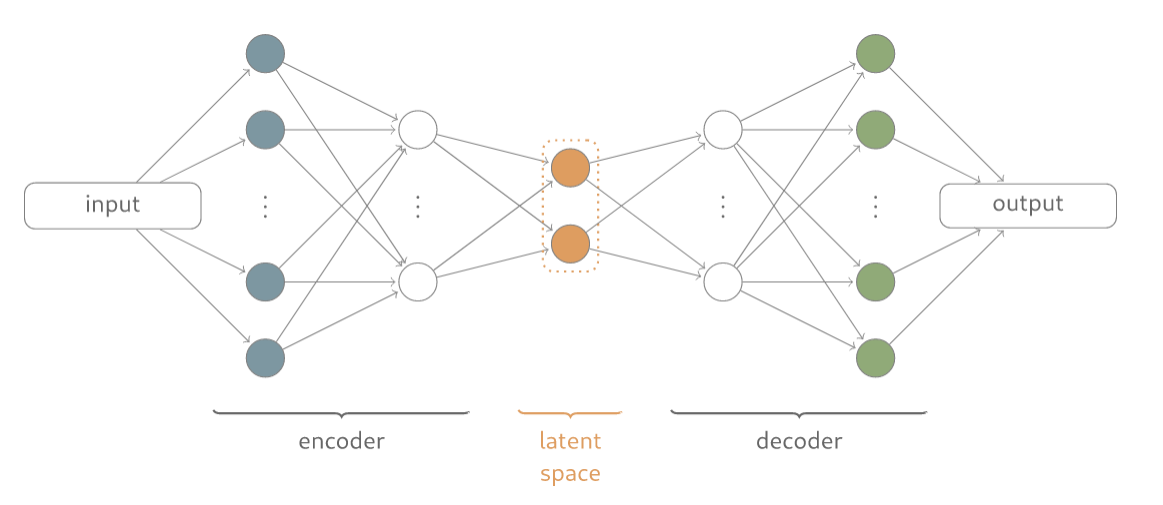
\includegraphics[width=1.0\textwidth,angle=0]{abb/ae_spinner}
    \caption[schematische Darstellung eines Autoencoders]{schematische Darstellung eines Autoencoders \cite{Spi2018}}
\end{figure}
Dies ist als eine Art Datenkompression zu sehen, da der Encoder spezifische Encodings generiert, die für die spätere Generierung der - dem orginalen Input sehr ähnlichen - Ausgabedaten nötig ist. Die Aufgabe des Encoders ist also, die Eingabedaten zu verarbeiten und sie einem Punkt im latenten Raum zuzuordnen. Als Verlustfunktion wird normalerweise entweder \frqq{mean-squared error\flqq} oder \frqq{cross-entropy\flqq} benutzt, um das Autoencoder-Netzwerk für Ausgaben zu bestrafen, die nicht den Eingaben entsprechen.
Da das Encoding bzw. der latente Raum sehr viel weniger Speicherplatz bedarf als die Originaleingabe, muss das Netzwerk Informationen verwerfen. Der Encoder lernt so viel wie nötig und so wenig wie möglich an relevanten Informationen im Encoding zu behalten, damit das Decodernetzwerk ein möglichst exaktes Abbild der Eingabedaten rekonstruieren kann \cite[S.64]{fos19}.
\begin{figure}[H]
    \centering
    
\includegraphics[width=1.0\textwidth,angle=0]{abb/autoencoder_standard}
    \caption[Funktionsweise eines Autoencoders]{Funktionsweise eines Autoencoders am Beispielbild der Zahl \frqq{5\flqq} aus dem MNIST-Set}
\end{figure}
Standard-Autoencoder können also kompakte Datenrepräsentationen lernen und ihre Eingabedaten sehr gut rekonstruieren. Sie können auch sehr gut zur Bildreinigung verrauschter Bilder verwendet werden, da der Encoder lernt, dass die Position des Rauschens innerhalb des latenten Raums nicht relevant ist. Das Problem mit Standard-Autoencodern ist im Hinblick auf generative Modelle, dass sie keine Interpolation im latenten Raum zulassen \cite{Spi2018}. Man möchte ja mit generativen Modellen nicht die Originaldaten wiederherstellen, sondern dem latenten Raum zufällige Stichproben entnehmen bzw. Variationen der Eingabedaten aus dem latenten Raum generieren. Wenn diese Stichproben in Raumdiskontinuitäten liegen, werden inkorrekte Ausgabedaten erzeugt, weil der Decoder schlichtweg keine Erfahrung mit Datenpunkten aus dieser Region des latenten Raumes hat.

\subsubsection{VAE}~\\
Variational Autoencoder haben hingegen einen \emph{kontinuierlichen} latenten Raum, welcher eine Interpolation und zufällige Stichproben erlaubt.
\begin{figure}[H]
    \centering
    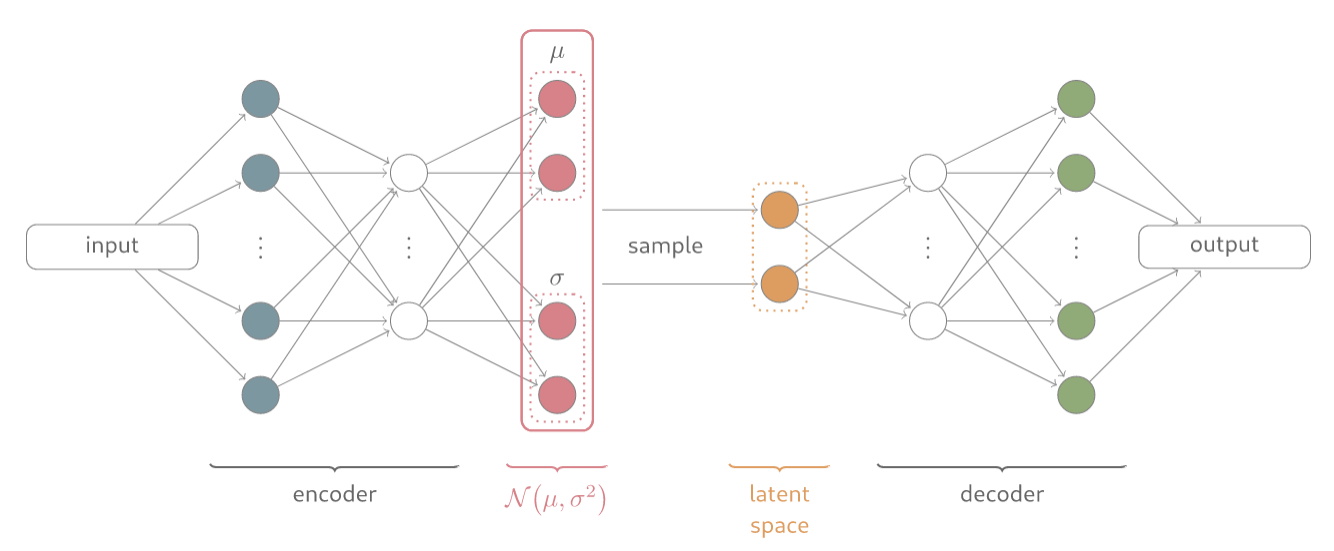
\includegraphics[width=1.0\textwidth,angle=0]{abb/vae_spinner}
    \caption[schematische Darstellung eines VAE]{schematische Darstellung eines VAE \cite{Spi2018}}
\end{figure}
Dies wird erreicht, indem der Encoder statt \emph{einem} Vektor der Größe $n$, \emph{zwei} Vektoren der Größe $n$ - $\mu$ und $\sigma$ - codiert. Dabei ist $\mu$ der Mittelwert der Verteilung und $\sigma$ der Logarithmus der Varianz jeder Dimension \cite{sha18}. In einem Standard-Autoencoder wird jedes Bild direkt auf einen Punkt im latenten Raum abgebildet. In einem VAE hingegen wird jedes Bild auf eine multivariate Normalverteilung um einen Punkt im latenten Raum abgebildet. Das bedeutet, dass der Encoder jede Eingabe zu einem Mittelwert- und einem Varianzvektor abbilden muss und sich nicht um die Kovarianz zwischen den Dimensionen zu sorgen braucht. Darüber hinaus ist $\sigma$ der Logarithmus der Varianz, da dieser eine beliebige reelle Zahl im Bereich ($-\infty, \infty$) annehmen kann, was dem natürlichen Ausgabebereich eines neuronalen Netzes entspricht, wohingegen die Varianz nur positive Werte annehmen kann \cite[S.81]{fos19}.
\begin{figure}[htb]
    \centering
    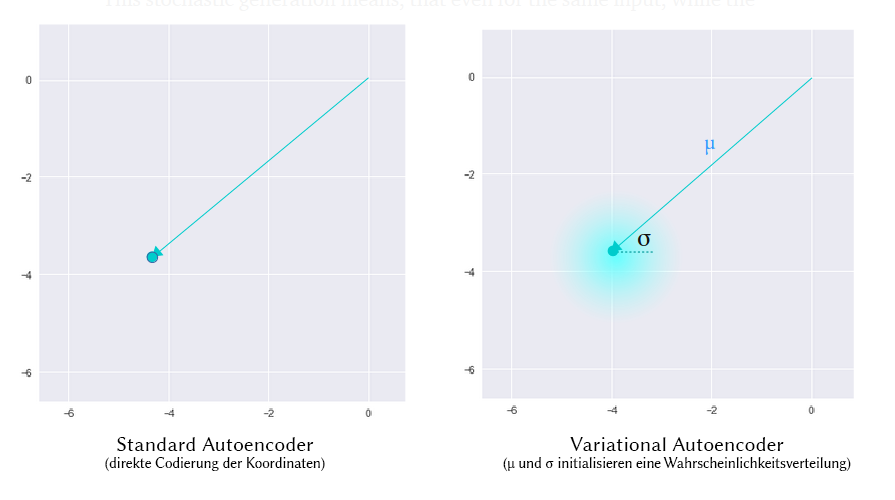
\includegraphics[width=0.9\textwidth,angle=0]{abb/VAE_muandsigma.png}
    \caption[Unterschied im Encoding - Autoencoder vs. VAE]{Unterschied im Encoding - Autoencoder vs. VAE \cite{sha18}}
\end{figure}
\FloatBarrier
Das Modell hat damit einen gewissen Grad an lokaler Variation im Encoding, jedoch keine überlappenden Cluster an variierenden Stichprobenencodings. Im Idealfall möchte man nicht nur im lokalen Stichprobenraum Variationen entnehmen, wo sich die Stichproben sehr ähnlich sind, sondern zwischen verschiedenen Klassen von Stichproben kontinuierlich interpolieren \cite{doe16}. Alle erkannten Merkmalcluster sollen also so nah wie möglich aneinander im latenten Raum angeordnet sein. Dies wird mit der Einrechnung der Kullback-Leibler-Divergenz in die Verlustfunktion erreicht \cite{sha18}. Die KL-Divergenz ist eine Methode, um zu messen, wie sehr sich eine Wahrscheinlichkeitsverteilung von einer anderen unterscheidet. Im Fall eines VAE soll gemessen werden, wie sehr sich die Normalverteilung mit den Parametern $\mu$ und $\sigma$ von der Standardnormalverteilung (Glockenkurve) unterscheidet. Das Netzwerk wird damit für die Codierung von Beobachtungen zu $\mu$ und $\sigma$ bestraft, die deutlich unterschiedlich von den Parametern einer Standardnormalverteilung sind \cite[S.102]{fos19}.
\begin{figure}[H]
    \centering
    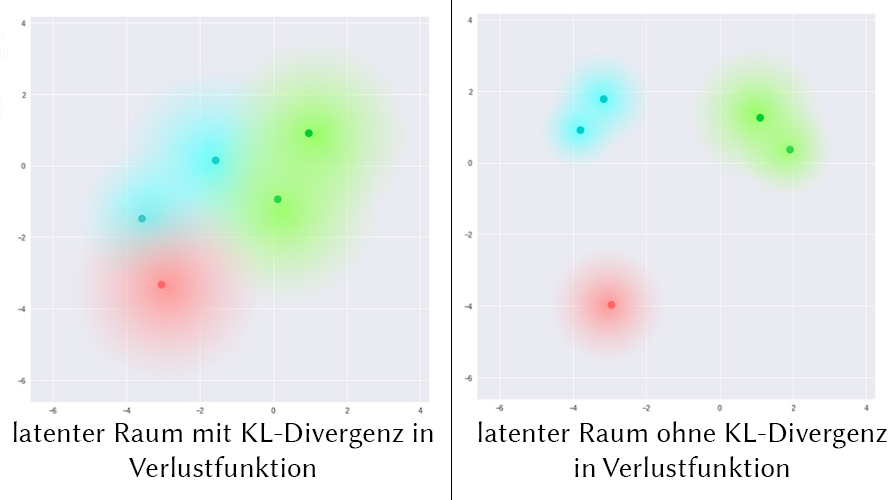
\includegraphics[width=0.7\textwidth,angle=0]{abb/VAE_KLL}
    \caption[Verteilung der Cluster mit und ohne KL-Divergenz]{Verteilung der Cluster mit und ohne KL-Divergenz \cite{sha18}}
\end{figure}
Mit einer optimierten Verlustfunktion und der KL-Divergenz können Verteilungen wie in Abbildung 2.6 erreicht werden.
\begin{figure}[H]
    \centering
    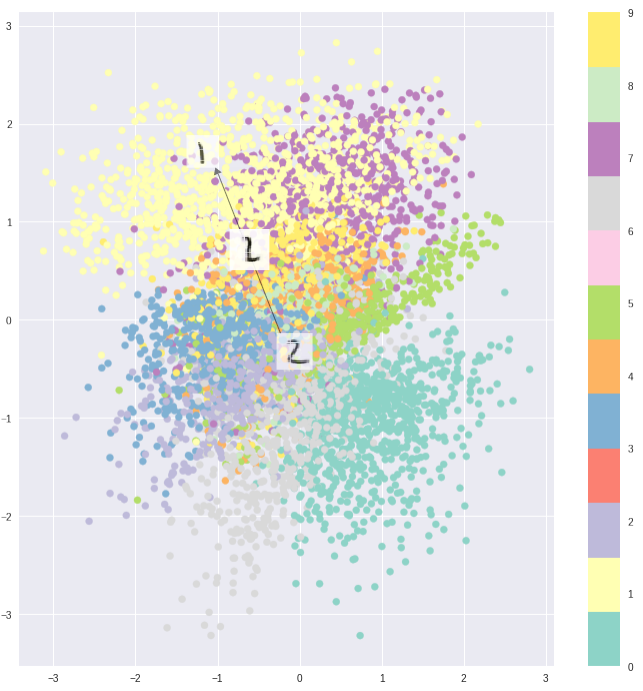
\includegraphics[width=0.6\textwidth,angle=0]{abb/vae_final.png}
    \caption[Verteilung im Encoding eines VAE]{Verteilung im Encoding eines VAE am Beispiel des MNIST-Sets \cite{sha18}}
\end{figure}


\subsection{Generative Adversarial Networks (GANs)}\label{Generative Adversarial Networks (GANs)}

Die GAN-Architektur für ein auf Deep Learning basierendes, generatives Modell wurde erstmals 2014 von Ian Goodfellow et al. auf der NIPS-Konferenz vorgestellt. Sie besteht aus zwei Submodellen:
\begin{itemize}
    \item Generator (G) - Modell, das neue Beobachtungen als Eingabedaten generiert
    \item Diskriminator (D) - Modell, das klassifiziert, ob die zugeführten Daten vom Trainingsset oder vom Generator stammen
\end{itemize}
Beide Modelle werden gleichzeitig trainiert. Der Generator versucht, Zufallsrauschen in Beobachtungen umzuwandeln, die so aussehen, als würden sie dem Trainingsdatensatz entstammen, und der Diskriminator versucht zu erkennen, ob eine Beobachtung aus dem ursprünglichen Datensatz stammt oder eine der Fälschungen des Generators ist \cite{bro19}. Am Anfang gibt der Generator sehr verrauschte Bilder aus und der Diskriminator prognostiziert zufällig. Der entscheidende Punkt von GANs ist, wie das Training der beiden Netzwerke abgewechselt wird, sodass, sobald der Generator geschickter im Täuschen des Diskriminators wird, dieser sich anpassen muss, um weiterhin die gefälschten Bilder zu erkennen. Das wiederum treibt den Generator dazu an, neue Wege zu finden, um den Diskriminator zu täuschen \cite[S.99]{fos19}.
\begin{figure}[H]
    \centering
    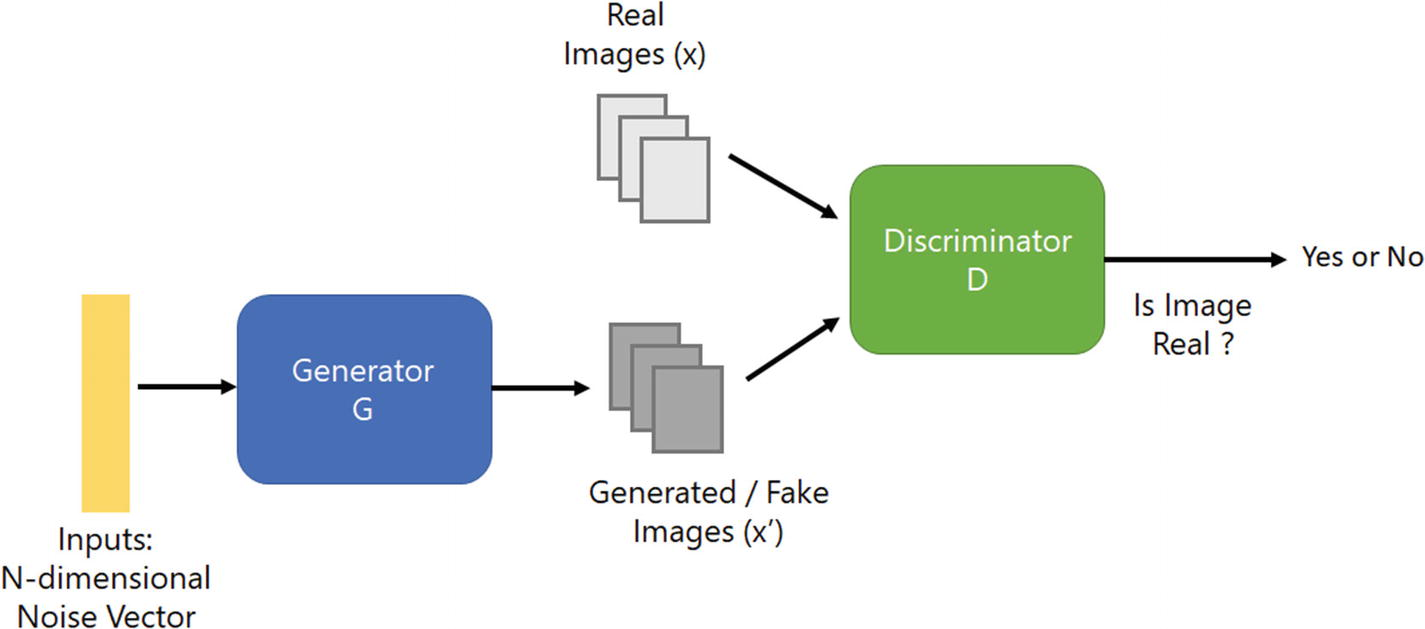
\includegraphics[width=1\textwidth,angle=0]{abb/Springer_GAN}
    \caption[Funktionsweise eines GAN]{Funktionsweise eines GAN \cite{SDT18}}
\end{figure}
Man kann sich das Training eines GAN als Nullsummenspiel vorstellen: Das Generatornetzwerk sei dabei ein Geldfälscher, der versucht, Falschgeld zu produzieren. Das Diskriminatornetzwerk sei die Polizei, die versucht, echtes Geld von gefälschtem Geld zu unterscheiden. Um das Spiel zu gewinnen, muss der Geldfälscher lernen, Geldscheine zu erzeugen, welche von echtem Geld ununterscheidbar sind\cite{goo16}. In diesem Fall bedeutet Nullsummenspiel, dass das jeweilige Netzwerk per Fehlerrückführung in jedem Trainingsschritt bestraft wird und dessen Modellparameter variiert werden. So entsteht nach sehr vielen Trainingsschritten ein generatives Modell, welches täuschend echte Daten generieren kann. Die GAN-Architektur wird vor allem bei der Generierung von Bilddaten verwendet.

Im Original-GAN-Forschungspaper von Ian Goodfellow et al. wurden dichte Schichten anstelle von Konvolutionsschichten für das Training verwendet. Seitdem hat sich jedoch gezeigt, dass Konvolutionsschichten dem Diskriminator eine bessere Vorhersagekraft verleihen. Diese Art von GANs wird in der Literatur auch DCGAN (Deep Convolutional Generative Adversarial Network) genannt. Heutzutage enthalten fast alle GAN-Architekturen Konvolutionsschichten, sodass das »DC« bereits enthalten ist, wenn über GANs geredet wird \cite{bro19}. Seit der ersten Vorstellung 2014 wurden bis heute mehr als 500 verschiedene Erweiterungen von GAN-Architekturen in wissenschaftlichen Papers vorgestellt. Diese haben verschiedene spezielle Eigenschaften, die zu einer verbesserten Lösung der jeweiligen Aufgabenstellung führt. Zwei der berühmtesten Erweiterungen von GANs sollen in dieser Seminararbeit erläutert werden.

\subsubsection{StyleGAN}~\\
In dem IEEE-Konferenzpaper \emph{\frqq{A Style-Based Generator Architecture for Generative Adversarial Networks}\flqq} wurde das Konzept des StyleGAN 2019 von Nvidia-Mitarbeitern vorgestellt. Die Bilder von menschlichen Gesichtern in Abbildung 2.8 wurden mit diesem generativen Modell erzeugt. StyleGAN besteht im Wesentlichen aus zwei Erweiterungen eines GAN:
Die Erzeugung hochauflösender Bilder durch PG-GAN (Progressively Growing GAN) und Einbindung von Stiltransfer durch AdaIN.
\begin{figure}[H]
    \centering
    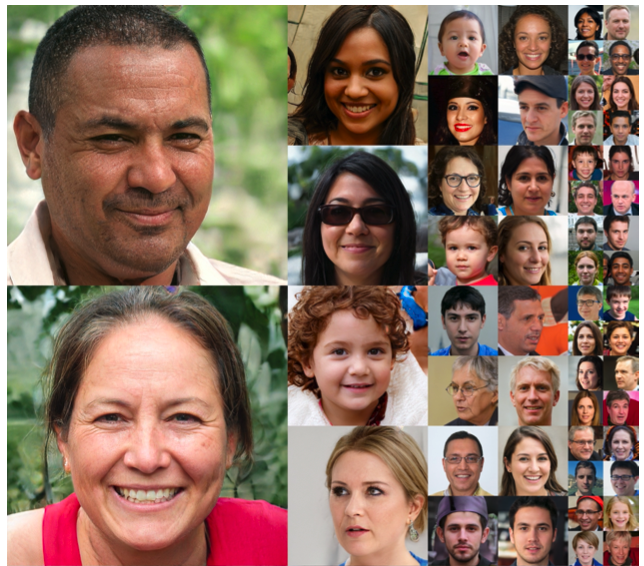
\includegraphics[width=0.6\textwidth,angle=0]{abb/StyleGAN_example_2}
    \caption[Beispielbilder StyleGAN]{Beispielbilder StyleGAN \cite{kar19}}
\end{figure}

\paragraph[]{PG-GAN}
\frqq{Progressives Wachstum\flqq} ist eine Methode zum Generieren von hochauflösenden Bildern. Ein PG-GAN fängt mit einer niedrigaufgelösten Repräsentation eines Bildes an und fügt im Trainingsprozess allmählich hochauflösendere Generatoren und Diskriminatoren hinzu. Im Schema in Abbildung 2.9 wird mit einer Auflösung von 4x4 begonnen und diese schrittweise auf 1024x1024 erhöht.
\begin{figure}[H]
    \centering
    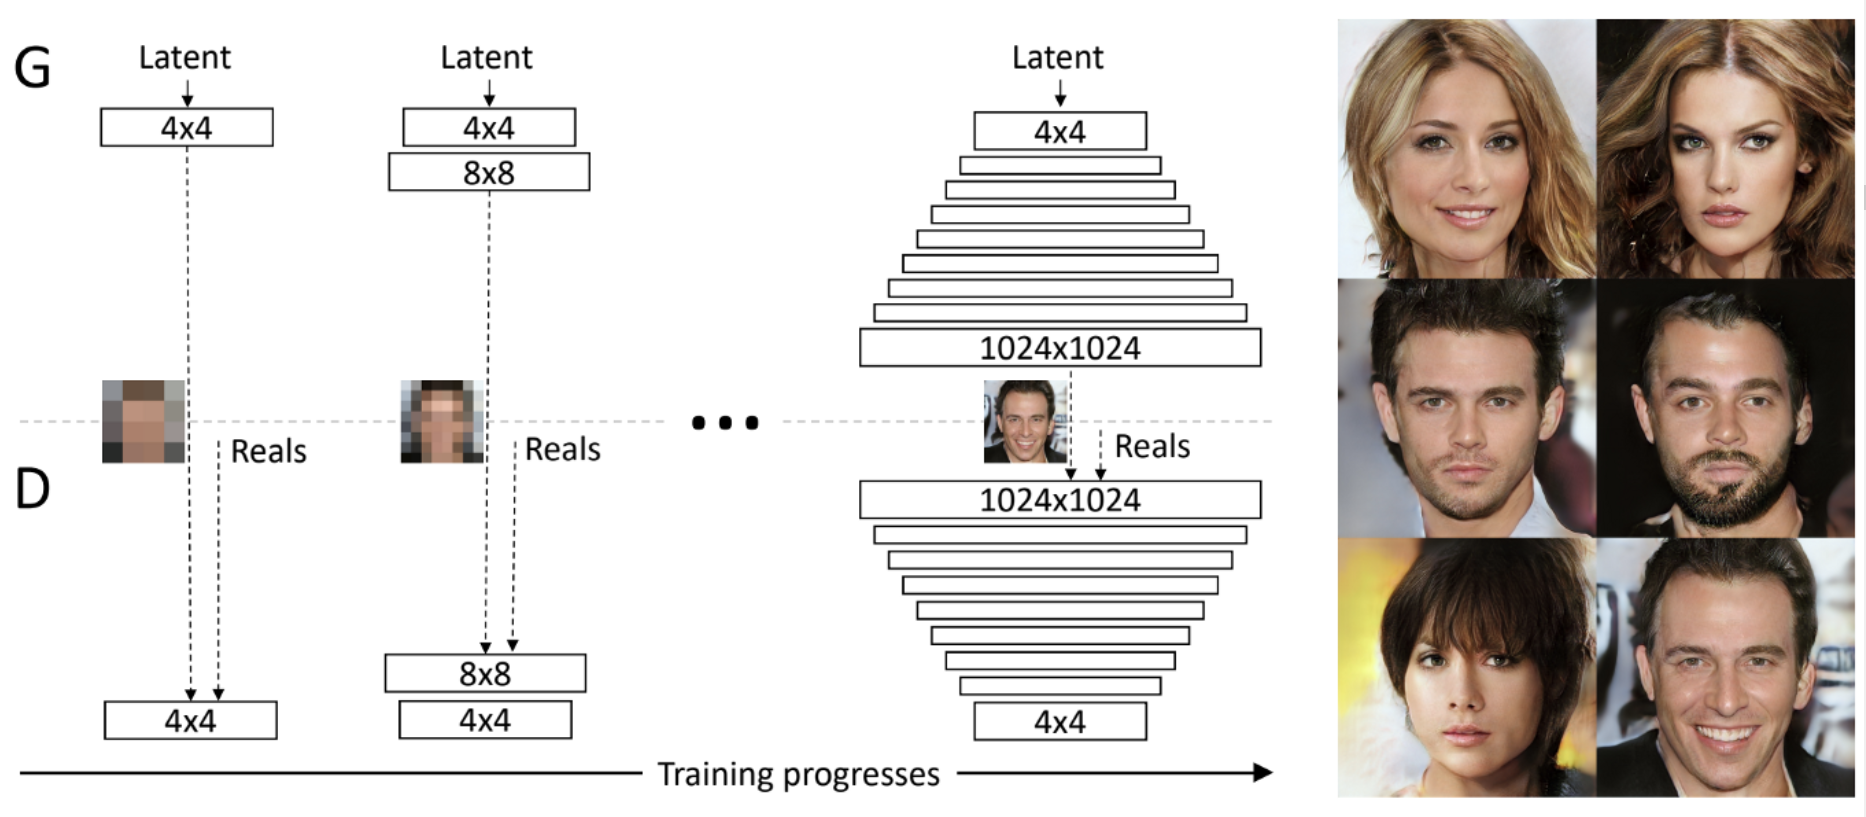
\includegraphics[width=1\textwidth,angle=0]{abb/pggan_schema}
    \caption[PG-GAN Schema]{PG-GAN Schema \cite{kar19}}
\end{figure}

\paragraph[]{AdaIN}
\frqq{Adaptive Image Normalization\flqq} (kurz AdaIN) ist ein Stiltransferalgorithmus und wurde 2017 von Xun Huang et al. vorgestellt. Im StyleGAN wird er als Normalisierungsmodul verwendet und in jeder Auflösungsebene des Generators im PG-GAN angewendet. AdaIN entspricht einer Art neuronaler Netzwerkschicht, die den Mittelwert und die Varianz der Ausgaben $x_i$ der einzelnen Feature-Maps aus einer jeweils vorgegebenen Schicht im Synthesenetzwerk mit einem Referenzstil-Bias $y_{b,i}$ und einer Skalierung $y_{s,i}$ anpasst. Die Stilparameter werden berechnet, indem zuerst ein latenter Vektor $z$ durch ein Mapping-Netzwerk $f$ geleitet wird, um einen Zwischenvektor $w$ zu erzeugen. Dieser wird dann durch eine dicht verbundene Schicht umgewandelt, um die Vektoren $y_{b,i}$ und $y_{s,i}$ mit jeweils einer Länge $n$ (der Anzahl der von der Konvolutionsschicht im Synthesenetzwerk ausgegebenen Kanäle) zu erzeugen. Dabei geht es vor allem darum, den Auswahlprozess des Stils für das Bild (das Mapping-Netzwerk) von dem eigentlichen Erzeugungsvorgang eines Bilds mit einem bestimmten Stil (das Synthesenetzwerk) zu trennen. Die adaptiven Instanz-Normalisierungsschichten stellen sicher, dass die Stilvektoren, die in jede Schicht eingespeist werden, nur Merkmale auf dieser Schicht beeinflussen, indem sie verhindern, dass Informationen bezüglich des Stils zwischen den Layern durchsickern \cite[S.277f]{fos19}.
\begin{figure}[H]
    \centering
    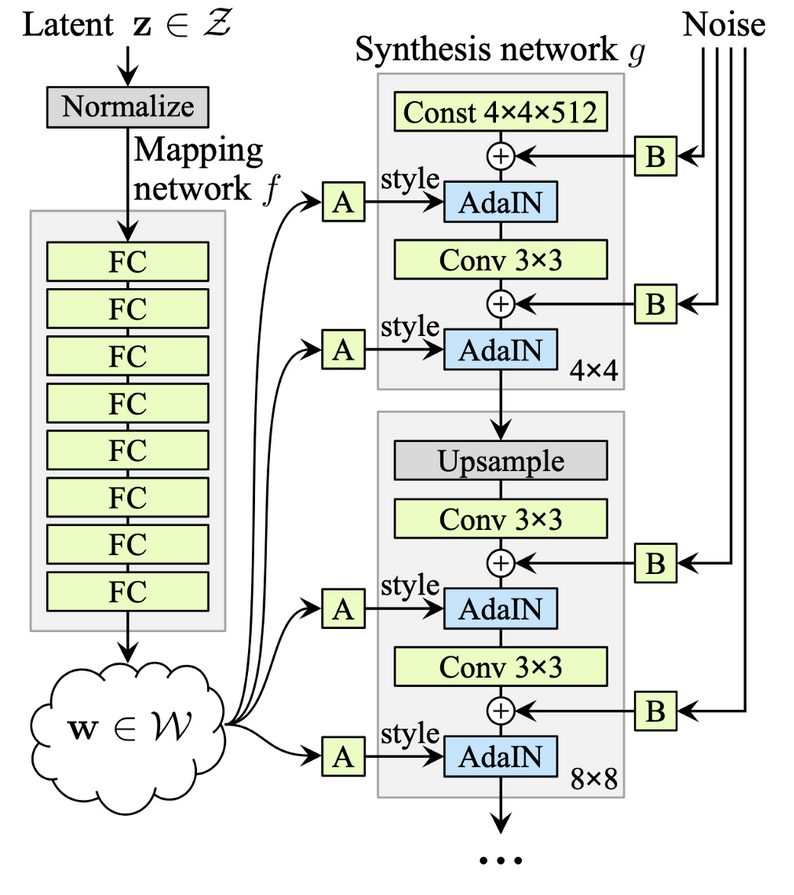
\includegraphics[width=0.6\textwidth,angle=0]{abb/adain_StyleGAN}
    \caption[Schema eines StyleGAN]{Schema eines StyleGAN \cite{kar19}}
\end{figure}

\subsubsection{CycleGAN}~\\
Das IEEE-Konferenzpaper von 2017 \cite{zhu17} stellte einen bedeutenden Fortschritt im Bereich des Stiltransfers dar. Es zeigt, wie ein Modell trainiert werden kann, das den Stil von einer Reihe von Referenzbildern auf ein anderes Bild überträgt, ohne einen Trainingssatz gepaarter Beispiele zu benötigen. Dies stellt eine Form des unüberwachten Lernens dar.
Ein CycleGAN generiert Bilder nicht aus Zufallsrauschen, sondern benutzt bereits vorhandene Bilder um eine neue Version der Bilder herzustellen. Diese sogenannte \frqq{Bild-zu-Bild Translation\flqq} erfolgt auf Basis des Bildinhalts auf der einen Seite, und des Bildstils auf der anderen. Die Trainingsdaten liegen also ungepaart aus zwei verschiedenen Domänen vor und müssen nicht über 1-zu-1-Zuordnungen verfügen. Das Netzwerk besteht aus zwei kombinierten GANs. Es nimmt ein Bild aus der Domäne $X$ als Input für den ersten Generator $G_X{\scriptscriptstyle\rightarrow}_Y$, dessen Aufgabe die Transformation eines Bildes der Domäne $X$ in die Zieldomäne $Y$ ist. Dieses neu generierte Bild wird dann Generator $G_Y{\scriptscriptstyle\rightarrow}_X$ zugeführt, welcher das Bild in ein Bild der Domäne $D_X$ zurückkonvertiert. Beide Generatoren haben korrespondierende Diskriminatoren, welche versuchen, die generierten Bilder von den Bildern ihrer jeweiligen Domäne zu unterscheiden \cite{zhu17}. Im genannten Paper wurde das Modell für 200 Epochen trainiert, um die Bildbeispiele in Abbildung 2.11 zu erhalten.
\begin{figure}[H]
    \centering
    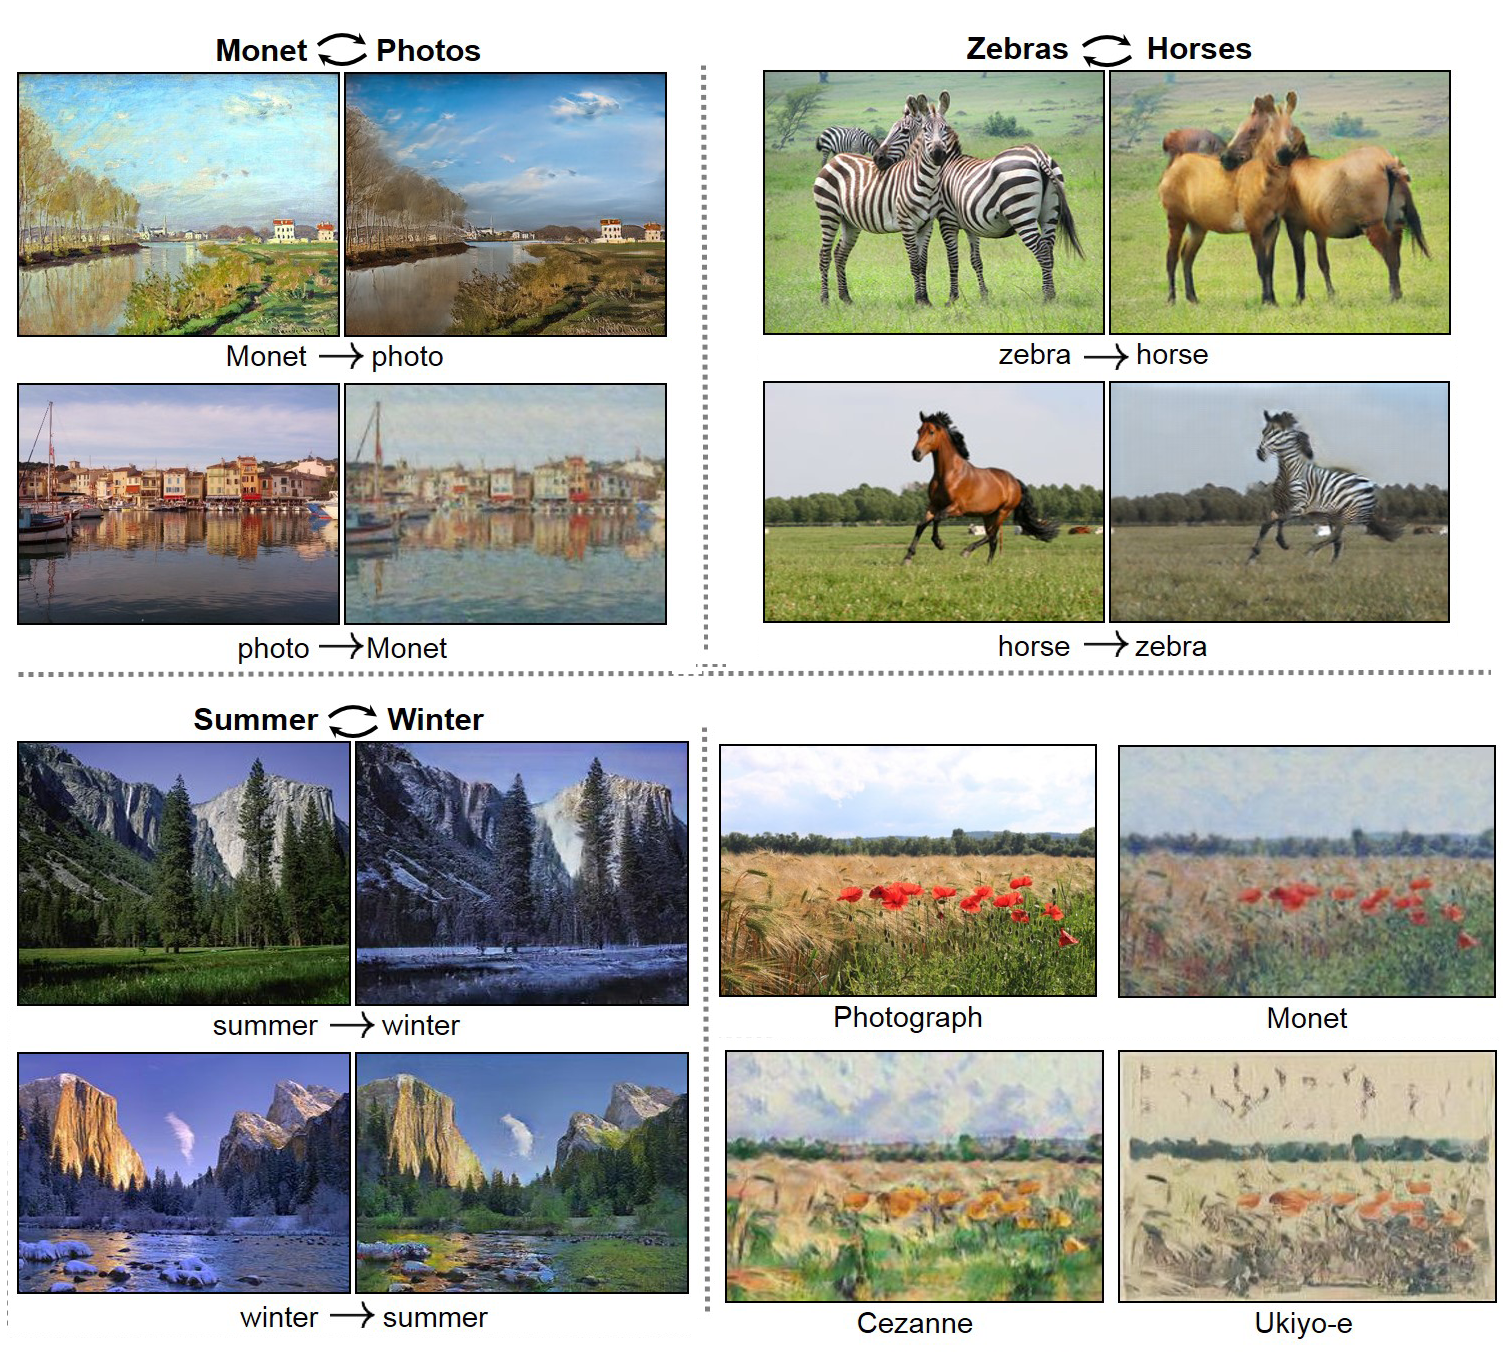
\includegraphics[width=0.8\textwidth,angle=0]{abb/CycleGAN_Beispiel}
    \caption[Beispiele von Stiltransfer mit CycleGAN]{Beispiele von Stiltransfer mit CycleGAN \cite{zhu17}}
\end{figure}
\newpage

\section{Anwendungsmöglichkeiten generativer Modelle}\label{Anwendungsmöglichkeiten generativer Modelle}

Im Gegensatz zu diskriminativen Modellen bieten generative Modelle kaum Lösungansätze für die Automatisierung von Validierungs- und Überwachungsprozessen in der Industrie. Generative Modelle eignen sich hingegen vor allem für die Erstellung von Inhalten wie Bilder, Texte oder Musik.
Deshalb liegt das größte Potenzial der Entwicklung in der Kreativbranche.

Bild
- Stiltransfer (aiportraits.com)
- Entrauschen ( Nvidia denoiser )
- SRGAN
- SyleGAN2 (thispersondoesnotexist.com)

Ton
-Stiltranfer
Text
\newpage

% hier können weitere Kapitel angelegt und eingetragen werden
% ....

\section{Ausblick}\label{ausblick}

Text des Ausblicks... Lorem ipsum dolor sit amet, consetetur sadipscing elitr, sed diam nonumy eirmod tempor invidunt ut labore et dolore magna aliquyam erat, sed diam voluptua. At vero eos et accusam et justo duo dolores et ea rebum. Stet clita kasd gubergren, no sea takimata sanctus est Lorem ipsum dolor sit amet. Lorem ipsum dolor sit amet, consetetur sadipscing elitr, sed diam nonumy eirmod tempor invidunt ut labore et dolore magna aliquyam erat, sed diam voluptua. At vero eos et accusam et justo duo dolores et ea rebum. Stet clita kasd gubergren, no sea takimata sanctus est Lorem ipsum dolor sit amet.


\newpage
\section{Fazit}\label{fazit}

Text des Fazits... Lorem ipsum dolor sit amet, consetetur sadipscing elitr, sed diam nonumy eirmod tempor invidunt ut labore et dolore magna aliquyam erat, sed diam voluptua. At vero eos et accusam et justo duo dolores et ea rebum. Stet clita kasd gubergren, no sea takimata sanctus est Lorem ipsum dolor sit amet. Lorem ipsum dolor sit amet, consetetur sadipscing elitr, sed diam nonumy eirmod tempor invidunt ut labore et dolore magna aliquyam erat, sed diam voluptua. At vero eos et accusam et justo duo dolores et ea rebum. Stet clita kasd gubergren, no sea takimata sanctus est Lorem ipsum dolor sit amet.

\cite{gfg14}
\cite{dtut16}
\cite{gfnips16}
\cite{rjVAE19}
\cite{rp_gml18}
\cite{o_pixel16}
\cite{sp17}
\cite{si18} 


%% Beispiel für Bild mit Fußnote
\begin{figure}[htb]
 \centering
 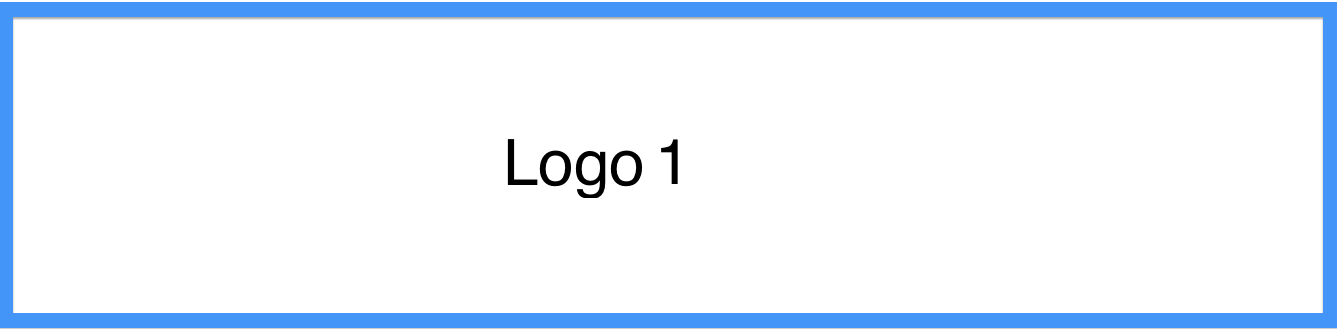
\includegraphics[width=0.4\textwidth,angle=45]{abb/logo1}
 \caption[Beispiel einer Bildbeschreibung]{Beispiel einer Bildbeschreibung\footnotemark}
\label{fig:beispiel1}
\end{figure}
\footnotetext{Bildquelle: Beispiel einer Bildquelle}

% Beispiel für Bildintegration
\begin{figure}[htb]
 \centering
 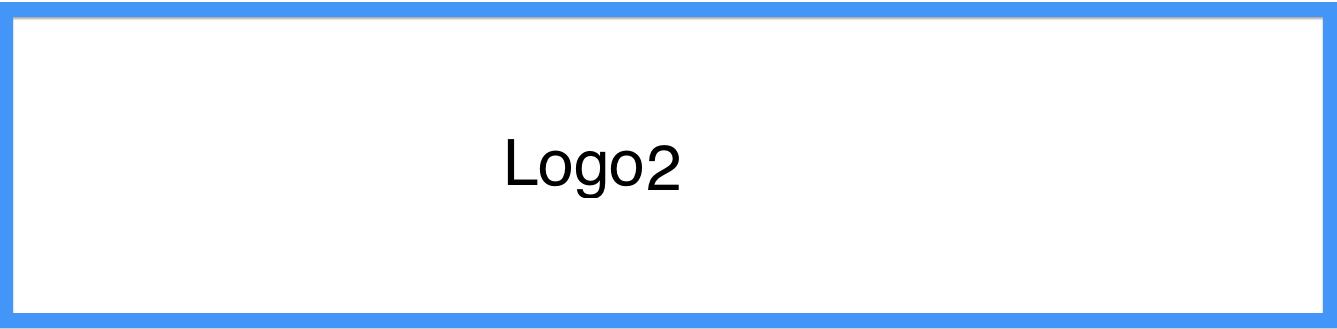
\includegraphics[width=0.3\textwidth,angle=0]{abb/logo2}
 \caption[Beschreibung]{Beschreibung}
\label{fig:Beschreibung}
\end{figure}

% Beispiel: Referenz auf Abbildung
Abbildung~\ref{fig:Beschreibung} [S.\pageref{fig:Beschreibung}]

% Beispiel: Tabelle 
\begin{center}
  \begin{tabular}{ | l | c | }
    \hline
    Überschrift 1 & Überschrift 2 \\ \hline \hline
    Info 1 & Info 2 \\ \hline
    Info 3 & Info 4 \\ \hline
    \hline
    \multicolumn{2}{|c|}{Info in einer Zelle} \\
    \hline
  \end{tabular}
\end{center}


% Beispiel für Quellcode Listings
\lstset{language=xml}
\begin{lstlisting}[frame=htrbl, caption={Die Datei {\normalfont \ttfamily  data-config.xml} dient als Beispiel für XML Quellcode}, label={lst:dataconfigxml}]
<dataConfig>
  <dataSource type="JdbcDataSource" 
              driver="com.mysql.jdbc.Driver"
              url="jdbc:mysql://localhost/bms_db"
              user="root" 
              password=""/>
  <document>
    <entity name="id"
        query="select id, htmlBody, sentDate, sentFrom, subject, textBody
        from mail">
    <field column="id" name="id"/>
    <field column="htmlBody" name="text"/>
    <field column="sentDate" name="sentDate"/>
    <field column="sentFrom" name="sentFrom"/>
    <field column="subject"  name="subject"/>
    <field column="textBody" name="text"/>
    </entity>
  </document>
</dataConfig>
\end{lstlisting}

\lstset{language=java}
\begin{lstlisting}[frame=htrbl, caption={Das Listing zeigt Java Quellcode}, label={lst:result2}]
/* generate TagCloud */
Cloud cloud = new Cloud();
cloud.setMaxWeight(_maxSizeOfText);
cloud.setMinWeight(_minSizeOfText);
cloud.setTagCase(Case.LOWER);
	    
/* evaluate context and find additional stopwords */
String query = getContextQuery(_context);
List<String> contextStoplist = new ArrayList<String>();
contextStoplist = getStopwordsFromDB(query);
	    
/* append context stoplist */
while(contextStoplist != null && !contextStoplist.isEmpty())
  _stoplist.add(contextStoplist.remove(0));
	    
/* add cloud filters */
if (_stoplist != null) {
  DictionaryFilter df = new DictionaryFilter(_stoplist);
  cloud.addInputFilter(df);
}
/* remove empty tags */
NonNullFilter<Tag> nnf = new NonNullFilter<Tag>();
cloud.addInputFilter(nnf);

/* set minimum tag length */
MinLengthFilter mlf = new MinLengthFilter(_minTagLength);
cloud.addInputFilter(mlf);

/* add taglist to tagcloud */
cloud.addText(_taglist);

/* set number of shown tags */	    
cloud.setMaxTagsToDisplay(_tagsToDisplay);
\end{lstlisting}


% Beispiel für Formeln
Die Zuordnung aller möglichen Werte, welche eine Zufallsvariable annehmen kann nennt man \emph{Verteilungsfunktion} von $X$.

\begin{quotation}
Die Funktion F: $\mathbb{R} \rightarrow$ [0,1] mit $F(t) = P (X \le t)$ heißt Verteilungsfunktion von $X$.\footnote{Mustermann, vgl.~\cite{mm2009}~[S.55]}
\end{quotation}

\begin{quotation}
Für eine stetige Zufallsvariable $X: \Omega \rightarrow \mathbb{R}$ heißt eine integrierbare, nichtnegative reelle Funktion $w: \mathbb{R} \rightarrow \mathbb{R}$ mit $F(x) = P(X \le x) = \int_{-\infty}^{x} w(t)dt$ die \emph{Dichte} oder \emph{Wahrscheinlichkeitsdichte} der Zufallsvariablen $X$.\footnote{Mustermann, vgl.~\cite{mf2005}~[S.56]}
\end{quotation}

% einfacher Zeilenabstand
\singlespacing
% Literaturliste soll im Inhaltsverzeichnis auftauchen
\newpage
\addcontentsline{toc}{section}{Quellenverzeichnis}
% Literaturverzeichnis anzeigen
\renewcommand\refname{Quellenverzeichnis}
\bibliography{Hauptdatei}

%% Index soll Stichwortverzeichnis heissen
% \newpage
% % Stichwortverzeichnis soll im Inhaltsverzeichnis auftauchen
% \addcontentsline{toc}{section}{Stichwortverzeichnis}
% \renewcommand{\indexname}{Stichwortverzeichnis}
% % Stichwortverzeichnis endgültig anzeigen
% \printindex

%\onehalfspacing
% evtl. Anhang
%\newpage
%\addcontentsline{toc}{section}{Anhang}
%\fancyhead[L]{Anhang} %Kopfzeile links
%\subsection*{Anhang}\label{anhang}

Der Anhang bestehend aus Bildern und Texten...

% Beispiel für Bildintegration
\begin{figure}[htb]
 \centering
 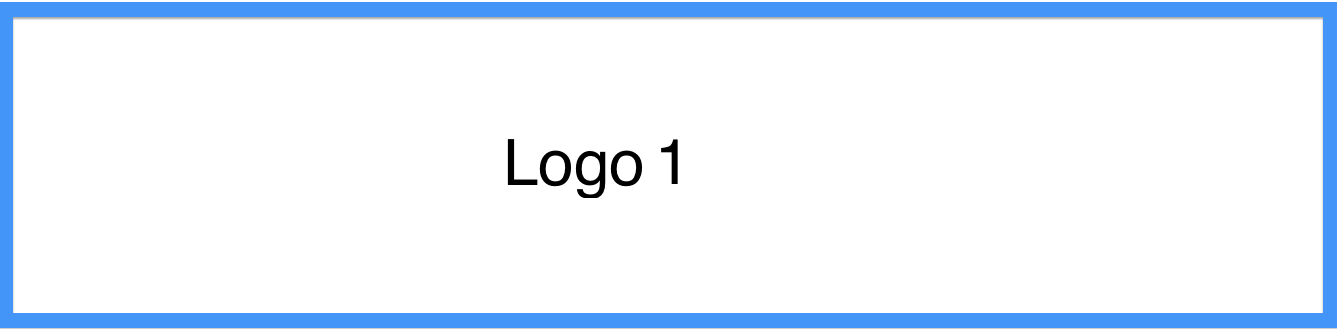
\includegraphics[width=0.3\textwidth,angle=0]{abb/logo1}
 \caption[Abbildung im Anhang]{Abbildung im Anhang}
\label{fig:Abbildung im Anhang}
\end{figure}

Lorem ipsum dolor sit amet, consetetur sadipscing elitr, sed diam nonumy eirmod tempor invidunt ut labore et dolore magna aliquyam erat, sed diam voluptua. At vero eos et accusam et justo duo dolores et ea rebum. Stet clita kasd gubergren, no sea takimata sanctus est Lorem ipsum dolor sit amet. Lorem ipsum dolor sit amet, consetetur sadipscing elitr, sed diam nonumy eirmod tempor invidunt ut labore et dolore magna aliquyam erat, sed diam voluptua. At vero eos et accusam et justo duo dolores et ea rebum. Stet clita kasd gubergren, no sea takimata sanctus est Lorem ipsum dolor sit amet.


% Eidesstattliche Erklärung
%\newpage
%\addcontentsline{toc}{section}{Eidesstattliche Erklärung}
%\section*{Eidesstattliche Erklärung}
\thispagestyle{empty}

\begin{verbatim}

\end{verbatim}

\begin{LARGE}Eidesstattliche Erklärung zur <-Arbeit>\end{LARGE}
\begin{verbatim}


\end{verbatim}
Ich versichere, die von mir vorgelegte Arbeit selbstständig verfasst zu haben. Alle Stellen, die wörtlich oder sinngemäß aus veröffentlichten oder nicht veröffentlichten Arbeiten anderer entnommen sind, habe ich als entnommen kenntlich gemacht. Sämtliche Quellen und Hilfsmittel, die ich für die Arbeit benutzt habe, sind angegeben. Die Arbeit hat mit gleichem Inhalt bzw. in wesentlichen Teilen noch keiner anderen Prüfungsbehörde vorgelegen.



\begin{displaymath}
% use packages: array
\begin{array}{ll}
Unterschrift:~~~~~~~~~~~~~~~~~~~~~~~~~~~~~~~~~~~~~~~~~~
& Ort, Datum:~~~~~~~~~~~~~~~~~~~~~~~~~~~~~~~~~~~~~~~~~~
\end{array}
\end{displaymath}


\end{document}
